% Created 2016-04-27 Wed 04:09
\documentclass[11pt]{article}
\usepackage[utf8]{inputenc}
\usepackage[T1]{fontenc}
\usepackage{fixltx2e}
\usepackage{graphicx}
\usepackage{grffile}
\usepackage{longtable}
\usepackage{wrapfig}
\usepackage{rotating}
\usepackage[normalem]{ulem}
\usepackage{amsmath}
\usepackage{textcomp}
\usepackage{amssymb}
\usepackage{capt-of}
\usepackage{hyperref}
\author{Pan An (A0134556A)}
\date{\today}
\title{Directional Dipole Model for Subsurface Scattering}
\hypersetup{
 pdfauthor={Pan An (A0134556A)},
 pdftitle={Directional Dipole Model for Subsurface Scattering},
 pdfkeywords={},
 pdfsubject={},
 pdfcreator={Emacs 24.5.1 (Org mode 8.3.4)}, 
 pdflang={English}}
\begin{document}

\maketitle
\tableofcontents


\section{Introduction}
\label{sec:orgheadline1}
Jensen et al. proposed a method for rendering the effects of 
subsurface scattering by using the Bidirectional Surface Scattering
 Reflectance Distribution Function (BSSRDF). 
Subsurface scatter- ing is caused when light scatters one
 to multiple times in a semi-translucent object,
 and is very important in a variety of different objects, such
 as milk or jade. Without this effect, rendered objects have a 
rough and hard computer generated feel to them.


This effect is simulated in a ray tracer by casting samples over the surface
 of the object and into the object. Original BSSRDF renders translucent materials 
using Monte Carlo ray tracing is computationally expensive 
due to a large number of subsurface scattering events.

This report is the implementation of an analytical model for subsurface scattering 
which captures translucency effects that are present in the reference solutions but 
remain absent with existing models. The idea is that a ray source corresponds better to 
the light that refracts through the surface of a translucent material.

This model is as time efficient as

\section{Related Work}
\label{sec:orgheadline2}
Subsurface scattering(SSS), is an optical physics based machanism describing the
process of light penetrating translucent materials. Different models
have been proposed in order to produce artifitial images of real life
materials. Bidirectional reflectance distribution~\cite{} function was
introduced as a simple but efficient model for reflection of light at
the surface of objects. Jensen et. al.~\cite{} introduced an improved model:
bidirectional subsurface scattering reflection distribution
function(BSSRDF).

A list of some physical caracteristics of different materials  has been
measured in Jensen's work. Gkioulekas et. al.~\cite{} studied on the
physical characteristics of daily materials. Gkioulekas et. al. used a
series of techniques and algorithms in order to achieve a set of data
for daily materials such as wine, milk, coffee etc. Based on their
analysis we are able to achieve a better result in multimedia
rendering.

\section{Platform and Frameworks}
\label{sec:orgheadline3}

My code is running on my personal computer, the specifications is listed:
\begin{center}
\begin{tabular}{lll}
\hline
\hline
Hardware & Params & Additional\\
\hline
CPU & i7 & \\
GPU & NVIDIA & GTX 780m\\
RAM & 16GB & \\
DRAM & 3GB & \\
\hline
\end{tabular}
\end{center}

Upenn(University of Pennsylvania) has open sourced one of their \href{https://cis565-fall-2015.github.io/}{framework}  for 
global illumination and rendering. My project is based on the ray tracing framework
of Upenn.


\section{Algorithm/Implementation}
\label{sec:orgheadline7}

\subsection{Ray Tracer}
\label{sec:orgheadline4}
Basic ray tracer model is used 
\subsection{Antialising}
\label{sec:orgheadline5}

\subsection{}
\label{sec:orgheadline6}

\section{Results}
\label{sec:orgheadline8}

\usepackage{subfig}
\begin{figure}
\centering
\subfloat[{$\ N = 100$}]{
  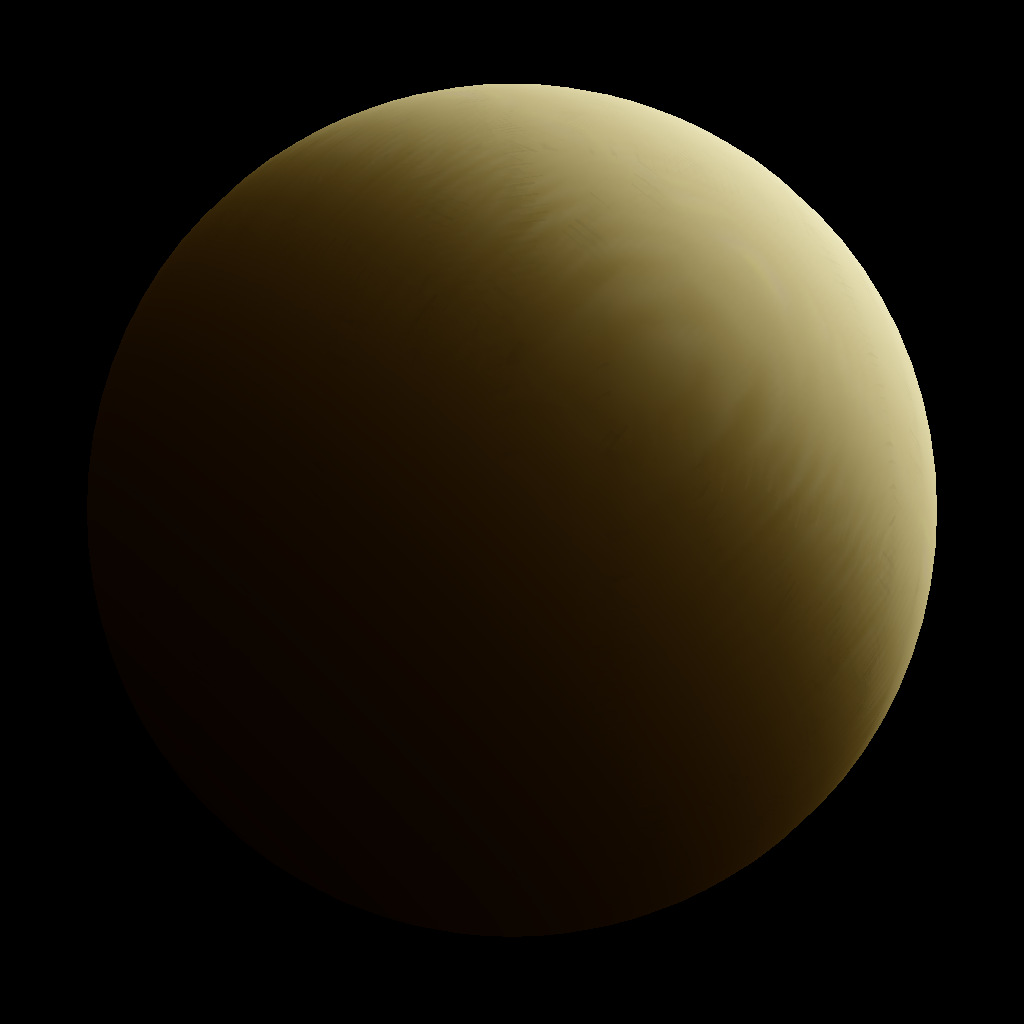
\includegraphics[width=0.15 \textwidth]{p100}
}
\subfloat[{$\ N = 1000$}]{
  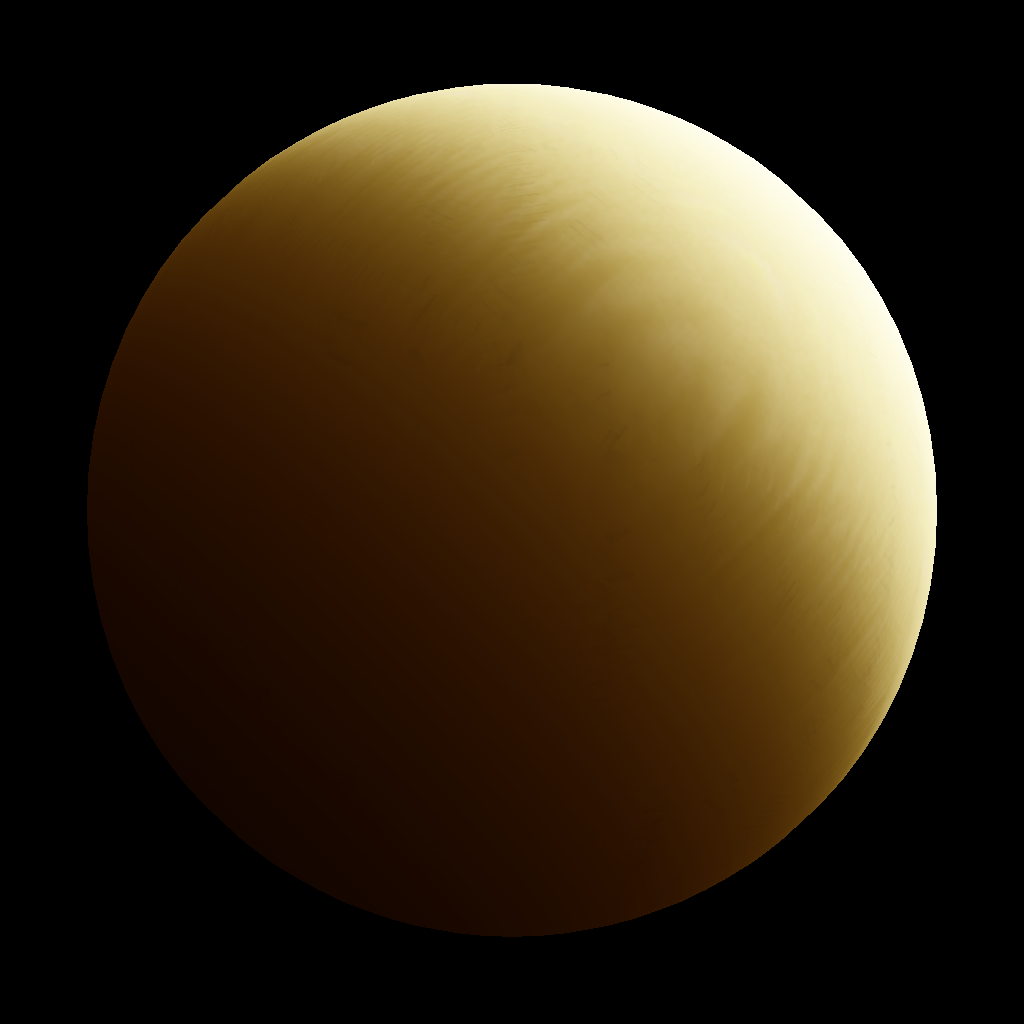
\includegraphics[width=0.15 \textwidth]{p1000}
}
\subfloat[$\ $Reference]{
  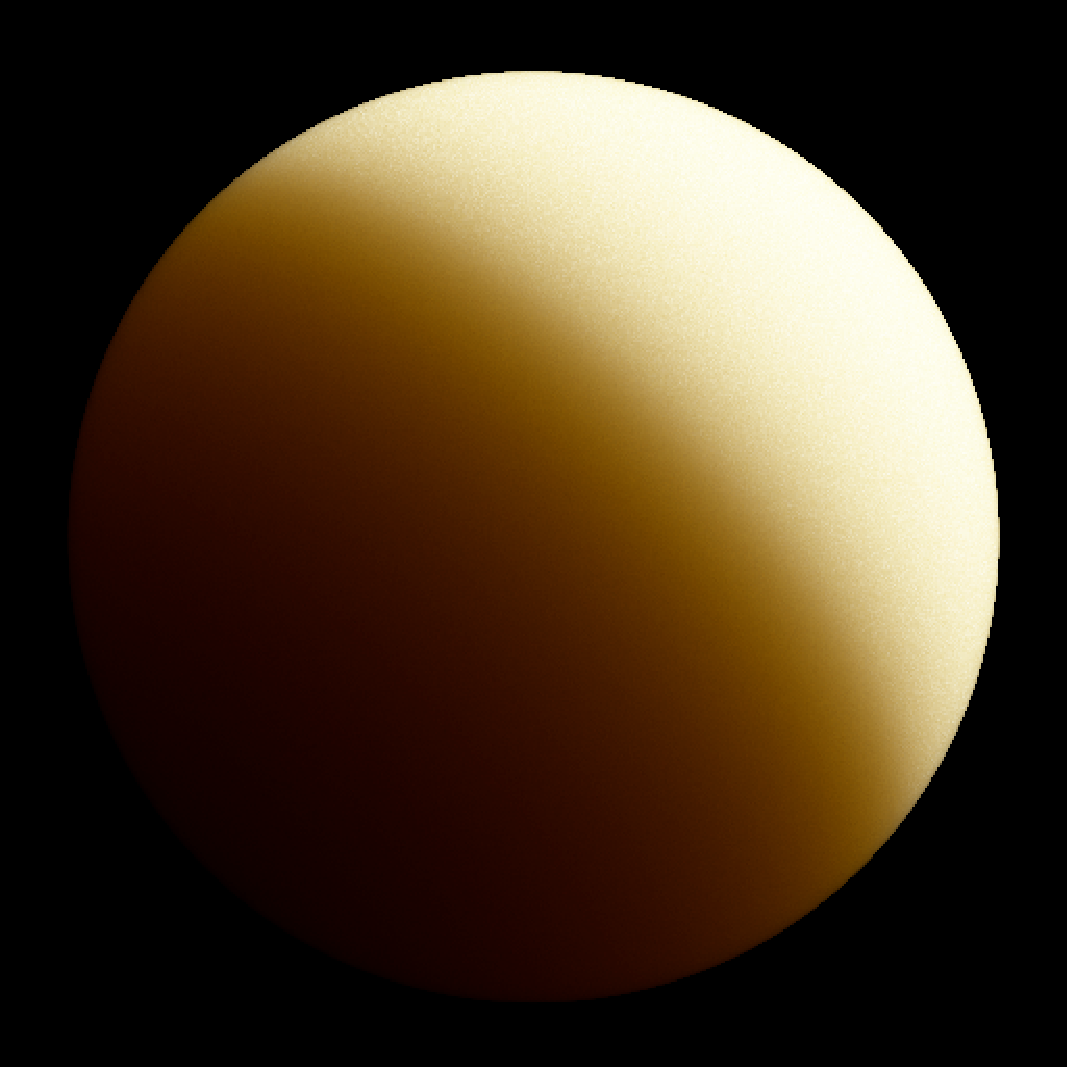
\includegraphics[width=0.15 \textwidth]{p}
} \\
\vspace{-0.4cm}
\subfloat[{$\ N = 100$}]{
  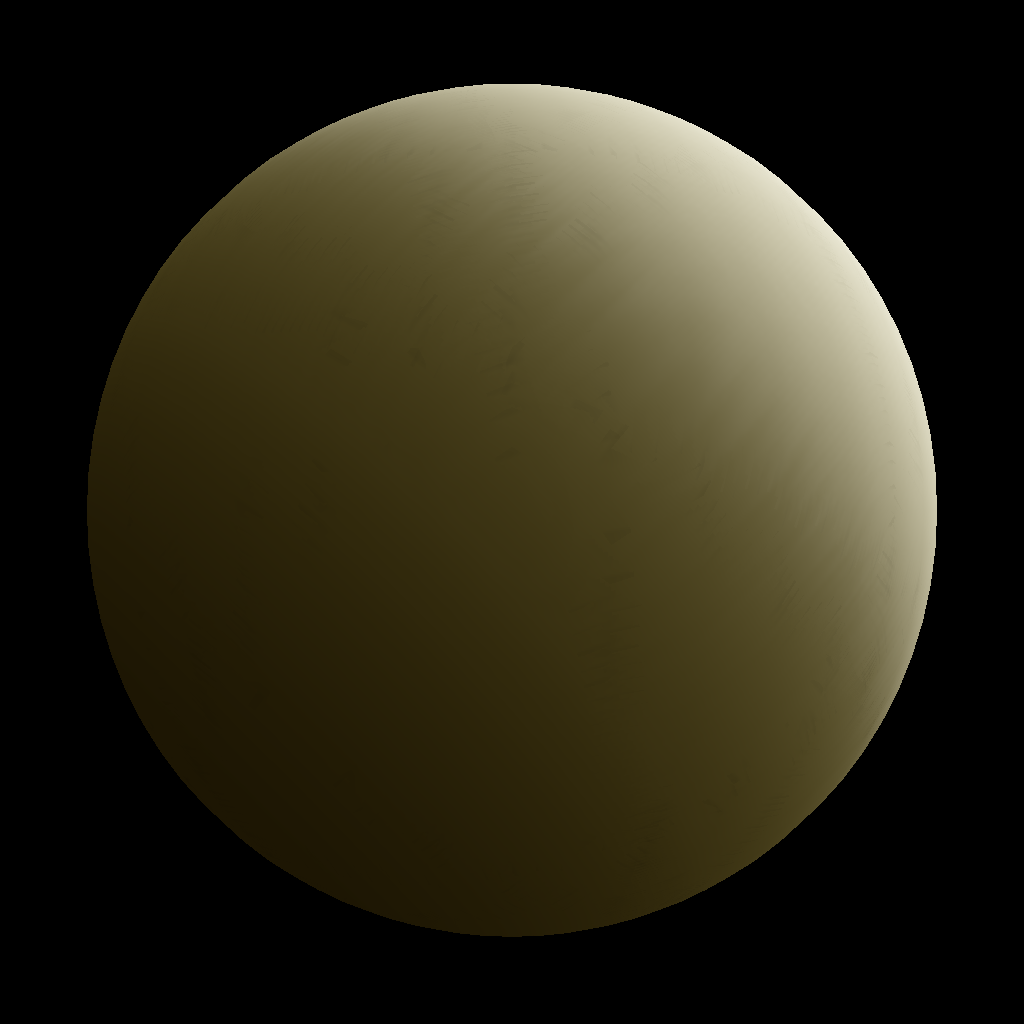
\includegraphics[width=0.15 \textwidth]{gj100}
} 
\subfloat[{$\ N = 1000$}]{
  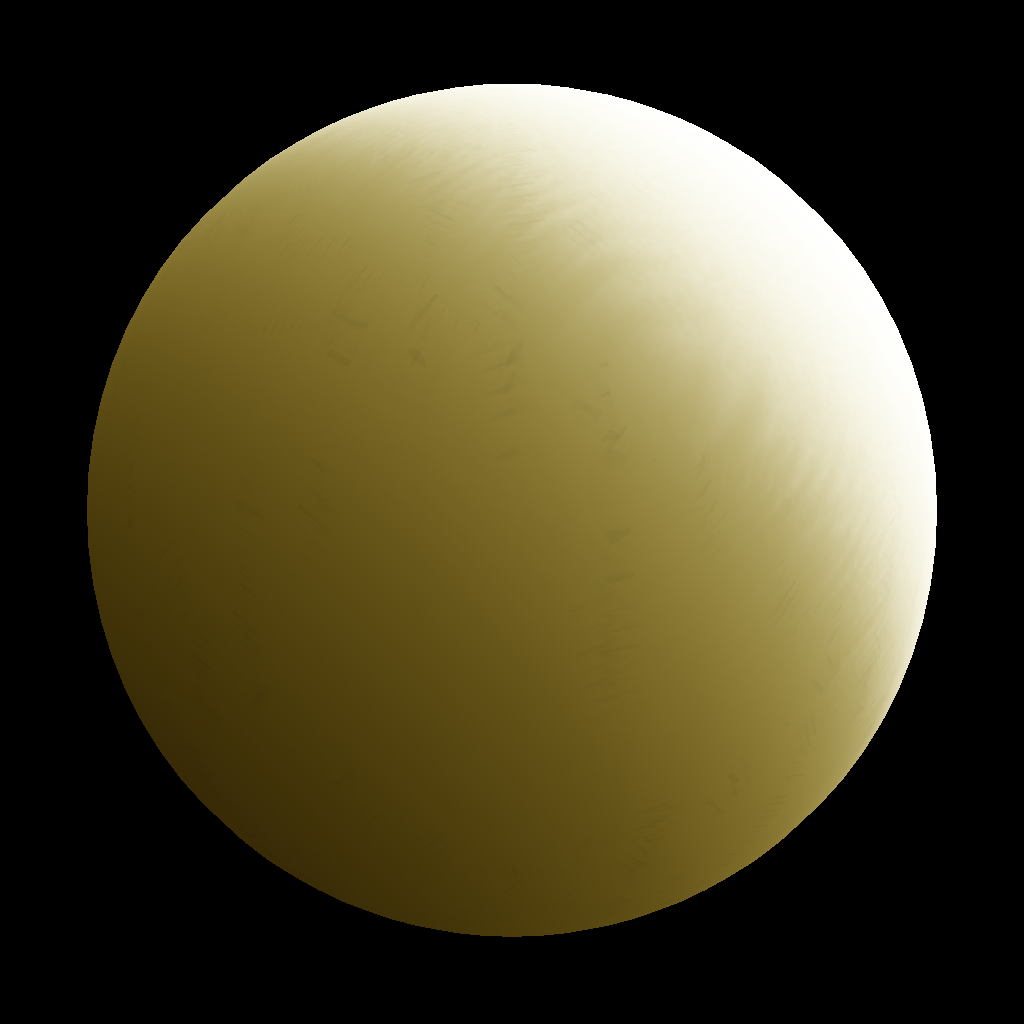
\includegraphics[width=0.15 \textwidth]{gj1000}
} 
\subfloat[$\ $Reference]{
  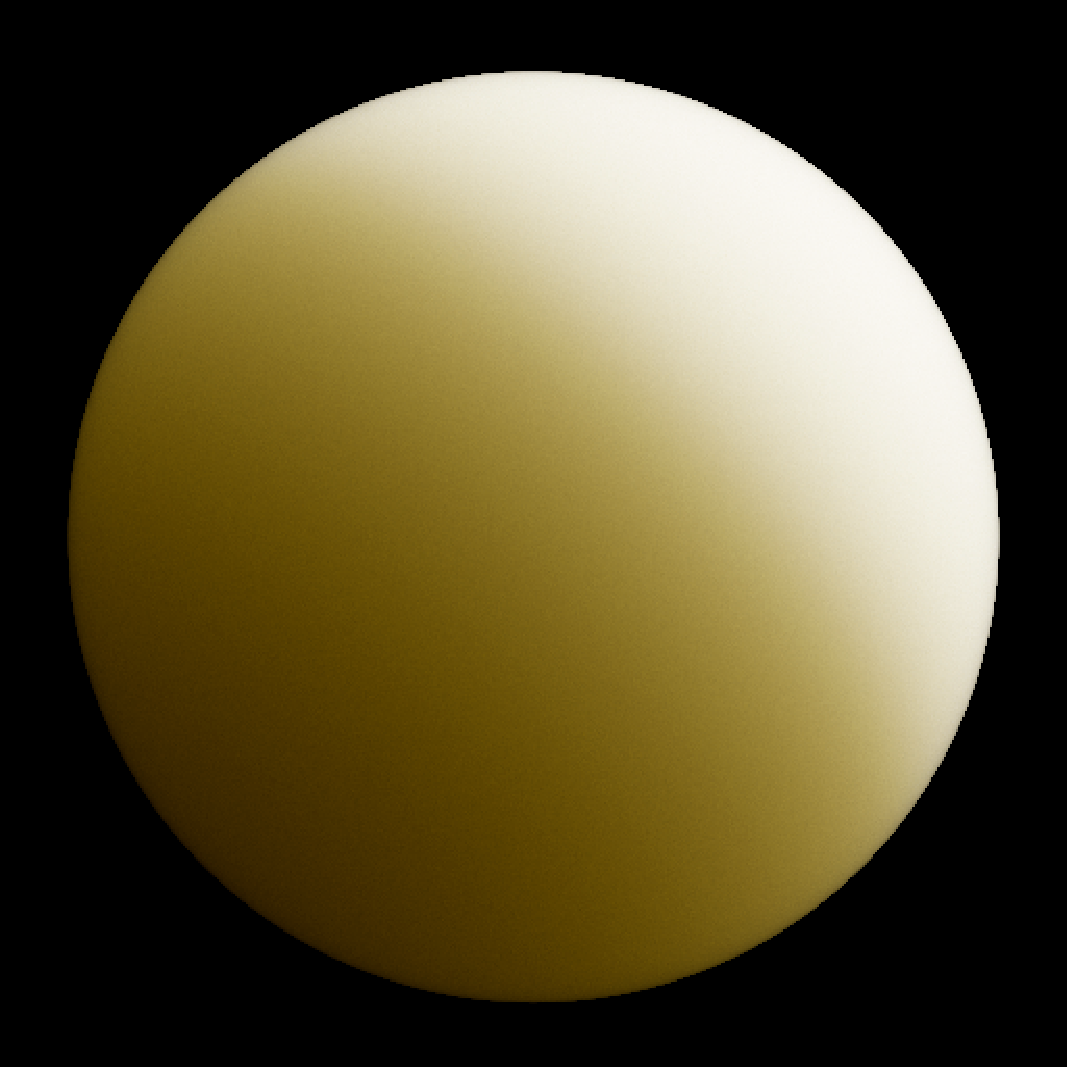
\includegraphics[width=0.15 \textwidth]{gj}
} 
\vspace{-0.2cm}
\caption{Comparazione dei risultati per patata e succo d'uva.}
\end{figure}


\section{Acknowledgements}
\label{sec:orgheadline9}

\section{References}
\label{sec:orgheadline10}
\end{document}
